\section{Розробка підходу до вирішення завдання}

\subsection{Огляд аналогів}
magic table

\subsection{Схема розв’язання}
% TODO: якось не consistently виходить. 
% TODO: Треба чітко розділити визначення capacity та задачу прогнозування як таку. ЗАПИТАТИ
% TODO: переробити перший розділ: частіше згадувати визначення пропускної здатності
% TODO: додати в другий розділ щось, де визначається пропускна здатність
Задача моєї дипломної роботи полягає в визначенні пропускної здатності маркетингового каналу. Для виконання задачі необхідно отримати перспективну інформацію щодо функціонування каналу та проаналізувати її. Схема розв’язання задачі зображена на рисунку \ref{fig:solution_schema}.

Пропонується прогнозувати діяльність маркетингового каналу за допомогою імітаційного моделювання. В перших двох діях на діаграмі активностей формулюються правила ділової гри та формується структура каналу, що дозволяє третьою дією побудувати імітаційну модель. Після того як модель побудована, можна запускати процес імітації (дія №4), який буде генерувати вихідні дані, що будуть проаналізовані: буде визначена пропускна здатність каналу.

% TODO: IDEF0 сюда!

%В даній роботі пропонується вирішувати задачу отримання перспективної інформації щодо функціонування маркетингового каналу за допомогою імітаційного моделювання, а саме: %побудувати мережу Петрі відповідно до структури каналу та автоматизувати ділову гру. 
%Задача:
% TODO: в чому задача: знайти пропускну здатність чи отримати перспективну інформацію? 

%Постановка задачі: розробки софта, моделювання
%1. Сформулювати правила гри
%2. Сформувати структуру каналу
%3. Побудувати імітаційну модель (мережу Петрі) 
%4. Провести імітацію
%5. Проаналізуівати отриману статистику -> визначити пропускну здатність каналу (приділити цьому увагу?)
%6. 
            \begin{stdfigure}
                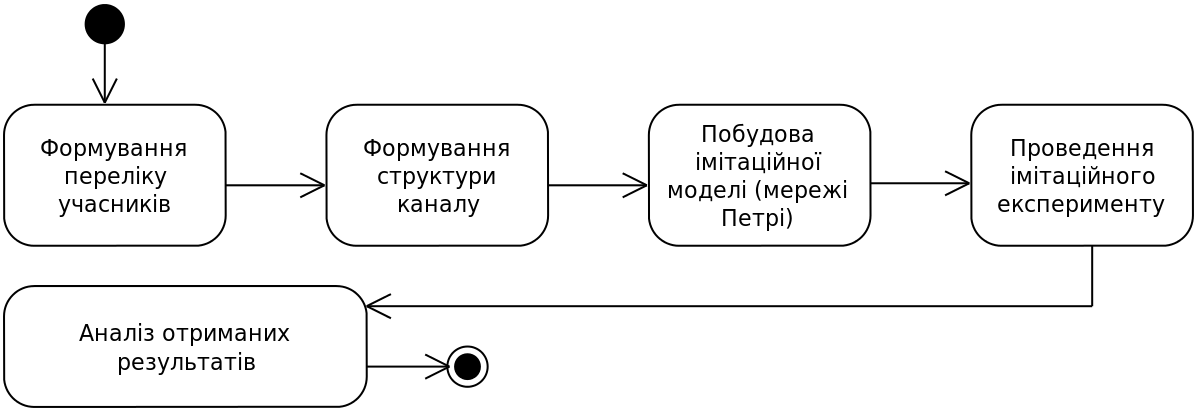
\includegraphics[width=7in]{images/uml_act_solution_schema.png}
                \caption{Схема вирішення задачі в вигляді діграми активностей}
                \label{fig:solution_schema}
            \end{stdfigure}   
% TODO: некрасивая
%\subsection{Теорія ігор}
%Что такое.
%Типы задач, способы описания задач.
%Решение задач.
% TODO: убрать теори игр? Зачем она?

%Деловая игра -- это игра с ненулевой суммой .... 
%Привести задачу одним из способов.
\subsection{Імітаційне моделювання}
\subsubsection{Огляд}
Моделювання --- це процесс побудови моделі для заміни досліджуємого об’єкту з метою дослідження його властивостей, прогнозування поведінки на основі властивостей моделі та характеристик її поведінки\cite{model}.

В залежності від характеру досліджуємих процесів всі види моделювання можуть бути розділені на:
\begin{enumerate}
\item детерміновані та стохастичні;
\item статичні та динамічні;
\item дискретні, безперервні та дискретно-безперервні;
\end{enumerate}

Детерміноване модeлювання відображає детерміновані процеси, тобто процеси, в яких передбачається відсутність будь-яких випадкових впливів; стохастичне моделювання відображає імовірнісні процеси та події. Статичне моделювання служить для описання поведінки моделі в будь-який момент часу, а динамічне відображає поведінку об’єкту в часі. Дискретне моделювання відображає дискретні процеси, а безперервне -- безперервні процеси\cite{model}.

Виділяють наступні основні методи моделювання\cite{model}:
\begin{longEnumerate}
   \item Математичне моделювання --- процес встановлення відповідності даному реальному об’єкту деякого математичного об’єкту, що називається математичною моделлю, та дослідження цієї моделі, що дозволяює отримувати характеристики об’єкта. 
   \item Аналітичне моделювання. В аналітичному моделюванні процеси записуються в вигляді функціональніх співвідношень та логичніх умов.
   \item Імітаційне моделювання. В цьому виді моделювання алгоритм, що реалізує модель, відтворює процес функціонування системи у часі.
   \item Комбіноване моделювання -- при будуванні комбінованих моделей для деяких складових процесу використовують аналітичні моделі, а для інших --- імітаційні.
\end{longEnumerate}

Імітаційне моделювання дозволяє досліджувати більш складні системи, ніж аналітичне моделювання. Імітаційна модель може відображати дискретність, нелінійність, недетермінованість та інші якості системи, які неможливо врахувати в аналітичних моделях. 
% TODO: дописать раздел

\subsubsection{Мережі Петрі}
Мережа Петрі --- це математичний апарат для моделювання динамічних дискретних систем. Мережею Петрі називають двудольний орієнтований граф \mbox {$ N = \langle P, T, * \rangle $}, де \mbox{$ P = \{p_i\}, T = \{t_i\} $} --- кінцеві непусті множини вершин, що називаються відповідно позиціями та переходами; $*$ --- відношення між вершинам, що відповідають дугам графа. Позиції зображаються кружками, переходи --- рисками. Дуги з’єднують кружки з рисками чи навпаки, але не вершини однакового типу.

Маркуванням мережі Петрі називається функція $Ф$, яка кожній позиції ставить в відповідність ціле позитивне не негативне число. Маркування характеризується вектором \mbox{$ F = \langle F(p_1), \dots, F(p_n) \rangle $}, де $n$ --- число позицій в мережі.

Різні маркування мережі Петрі хараактеризують стани відповідної динамічної системи, де динаміка моделюється рухом меток по позиціях.

Якщо кожна з вхідних позицій перехода $t$ складається з якомога однією мітки, то перехід $t$ може спрацювати. При спрацюванні переходу з кожної його вхідної позиції видаляється одна мітка, а в кожну вихідну додається.

            \begin{stdfigure}
                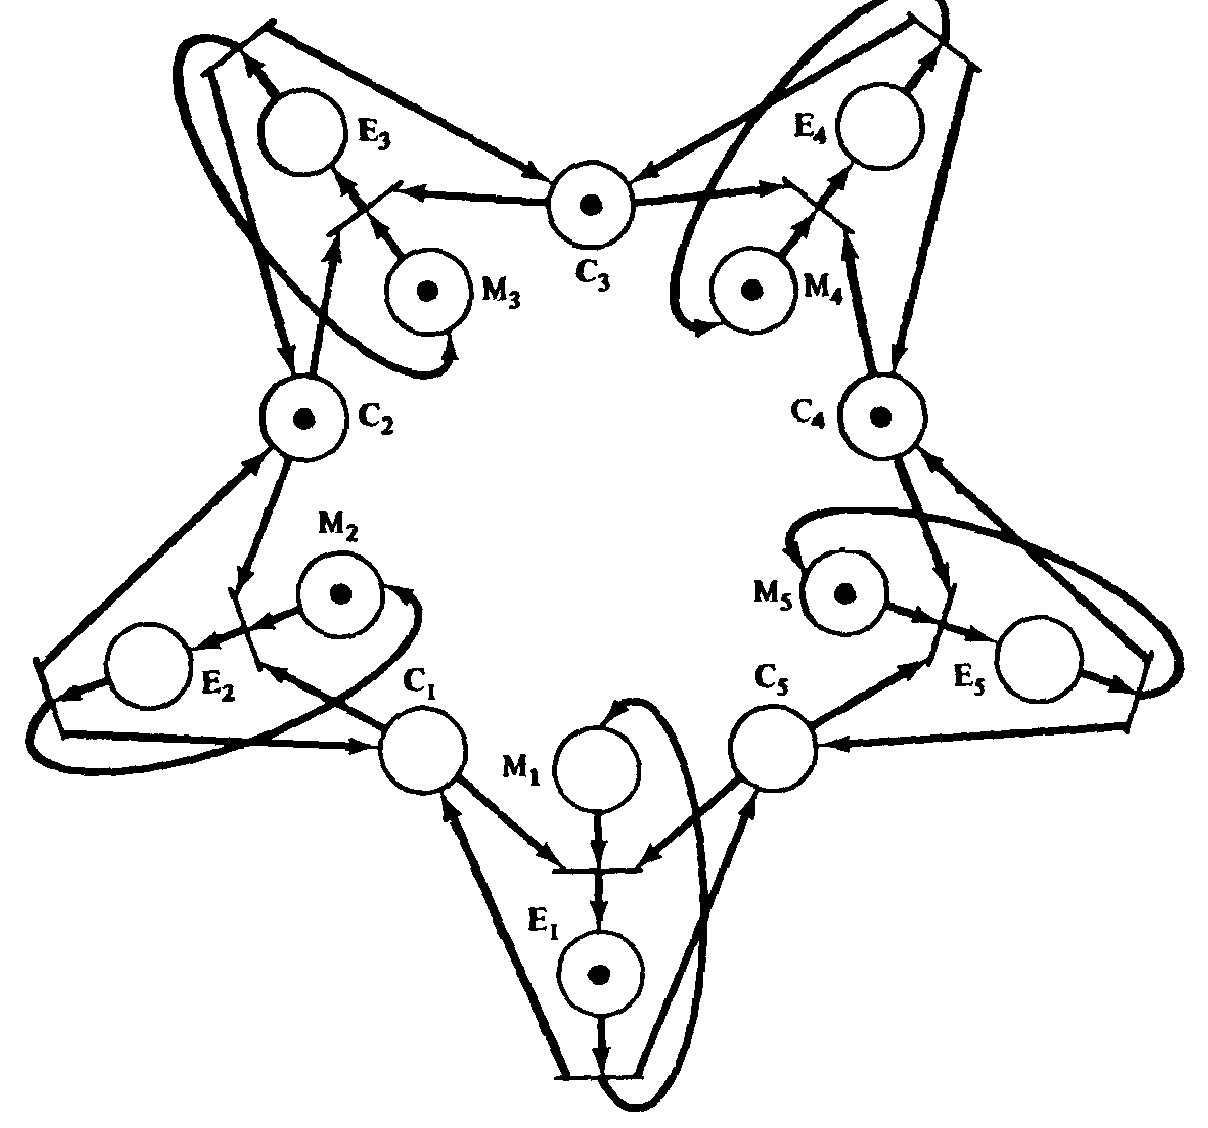
\includegraphics[width=4in]{images/petri_net_example.png}
                \caption{Приклад мережі Петрі}
                \label{fig:petri_net_example}
            \end{stdfigure}   

% Алгоритм построение модели! Сама игра -- єто процесс имитации.
% Позиція відображає дію -- замовлення, виробництво.
% Перехід відображає перехід ходу
% безпечні мережі петри
% TODO: побудувати модель саме тут!
%При применении сетей Петри для целей управления позициям сопос­
%тавляются операции (действия), а переходам — условия, при выполнении
%которых возбужденные переходы срабатывают, активизируя соответству­
%ющие операции [31]. При этом попадание меток в позицию ассоциируется
%с началом операции, а удаление метки — с ее окончанием. При исполь­
%зовании такого предположения считают, что любая операция не может
%быть повторно начата до ее завершения. Для описания таких процессов
%могут применяться только б е з о п а с н ы е сети Петри, т. е. такие сети, в
%которых при любой маркировке в каждой позиции не может быть более
%одной метки.

\subsection{Теорія ділових ігор}
	Якісь схеми ігор. Деловая игра -- это такая большая имитационная модель.



\subsection{Виводи до розділу}
Обосновать выбор.
